% Template for ICASSP-2018 paper; to be used with:
%          spconf.sty  - ICASSP/ICIP LaTeX style file, and
%          IEEEbib.bst - IEEE bibliography style file.
% --------------------------------------------------------------------------
\documentclass{article}
\usepackage{spconf,amsmath,graphicx}
\graphicspath{{images/}}

% Example definitions.
% --------------------
% \def\x{{\mathbf x}}
% \def\L{{\cal L}}

\title{Prosody Feature Extraction for Speech-To-Speech Synthesis}
\name{Jared Samet - UNI: jss2272}
\address{Columbia University SEAS\\
Data Science Institute - MS Program}
\begin{document}
%\ninept
%
\maketitle
%
\begin{abstract}
We present a system that extracts prosody features from a multi-speaker dataset.
The prosody features are computed by fitting low-degree Legendre series to the pitch and power contours of the audio for each vowel in the input audio.
Unsupervised clustering of the prosody features produces a discrete set of categories for the pronunciation of English vowels. A single-speaker speech dataset is annotated with cluster labels and used to train Tacotron, a neural-network based speech synthesis system.
By adding the cluster labels as annotation to text, the model can learn to incorporate prosody into its output.
The resulting system can produce audio that is different even when the text is the same.
By annotating the utterance of a new speaker, the trained speech synthesis model can produce new synthesized audio that, to a limited degree, mimics the prosody of the input.
\end{abstract}
%
\begin{keywords}
Prosody, pitch accent, vowels, clustering, speech synthesis
\end{keywords}
%
\section{Introduction}
\label{sec:intro}

A single English sentence can be pronounced in many different ways.
These different pronunciations can convey information above and beyond the actual words that are spoken.
Understanding prosody, also known as suprasegmental features, offers the potential for improved performance both in speech recognition and speech synthesis.
On the speech recognition side, a superior understanding of prosody may help a system respond more appropriately to spoken input.
On the output side, a speech synthesis system that could incorporate prosody features would have a wider expressive range and might be able to produce more natural sounding speech, or speech that had a more appropriate pronunciation for a given situation.

Pure text-to-speech systems, by definition, must produce a single pronunciation for a single sentence since the only input is the text.
In this project we demonstrate that certain aspects of prosody can be incorporated into a speech synthesis system to produce new synthesized audio that, to a certain degree, mimics the prosody of an input utterance.
To do this, we construct a set of features that can be represented compactly and that generalize well across multiple speakers.
We test the system by recording audio pairs of the same sentence pronounced in different ways and producing pairs of synthesized speech that differ only in the ways in which the words are pronounced.

\section{Related Work}
\label{sec:sota}

This project involved two main components: first, extracting prosody features from a set of input audio files; and second, training a text-to-speech synthesis model on a dataset that had been labeled using the extracted prosody features.

Selkirk \cite{selkirk1995sentence} discusses sentence prosody and pitch accent in the context of English. Ghahremani et al. \cite{ghahremani2014pitch} describes a pitch-extraction algorithm (``the Kaldi pitch tracker'') based on Talkin \cite{talkin1995robust} that is specifically designed for use in the speech recognition concept and is implemented in the open-source Kaldi project \cite{Povey_ASRU2011}. Fujisaki \cite{fujisaki2004information} models the $F_0$ contour over the duration of an utterance as the sum of a set of impulse response and step response functions, parameterized with a finite number of scalar values.
Wang et al. \cite{wang2008mandarin} use the pitch and amplitude contours to improve tone recognition in Mandarin by identifying ``maxima, minima, and inflection points of particular acoustic events.''
Wong and Siu \cite{pui2004decision} use robust regression and orthogonal polynomials to create features for a decision tree classifier in order to recognize tones in Chinese languages. Finally, Lin \cite{lin2005language} and Mary \cite{mary2011extraction} use a small number of Legendre polynomial coefficients to represent the pitch contour as a finite-dimensional feature vector, which is the approach used in this project.

Speech synthesis or text-to-speech is a well-studied problem that has been actively researched since the 1950s. While current commercial systems described in Khan et al. \cite{khan2016concatenative} and Taylor \cite{taylor2009text} generally use concatenative speech synthesis to produce their output, the alternative approach of parametric synthesis using neural networks is rapidly gaining popularity. Several papers since 2016 have demonstrated impressive results in the quality of the output.
The first of this generation was Google's WaveNet (Oord et al. \cite{oord2016wavenet}), followed in quick succession by Deep Voice and Deep Voice 2 from Baidu (Arik et al. \cite{arik2017deep}, \cite{arik2017deep2}), Char2Wav from MILA (Sotelo et al. \cite{sotelo2017char2wav}), and Tacotron from Google (Wang et al. \cite{wang2017tacotron}).
Each of these systems has taken a different approach to the network architecture to address different aspects of the speech synthesis pipeline. Tacotron, which is the backend used here, is an end-to-end text-to-speech system based on the sequence-to-sequence with attention model. Its design made it surprisingly simple to incorporate the prosody features described below.

\section{Overview}
\label{sec:overview}
The goal of this project was to create a system that, given an input audio file from an arbitrary speaker, produces a synthesized audio output of the same utterance in the voice of a second speaker, where the prosody of the output audio matches that of the input audio as closely as possible.
The system implemented uses a pipeline of several processing steps in order to accomplish this.
An overview of the pipeline and a diagram are presented here for context; a detailed description of each step follows.

\begin{figure}[htb]

\begin{minipage}[b]{1.0\linewidth}
  \centering
  \centerline{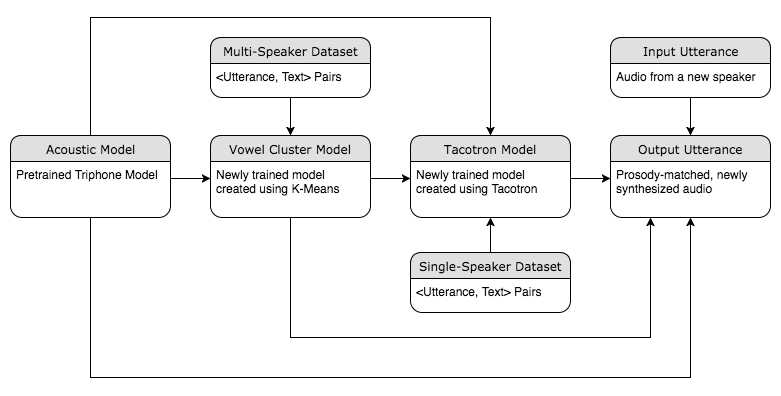
\includegraphics[width=8.5cm]{Overall_Pipeline}}
\end{minipage}
\caption{Pipeline Overview}
\label{fig:overview}
\end{figure}

The first portion of the system is the vowel-cluster training process, which takes as input a previously-trained acoustic model for alignment and a speech dataset from multiple speakers. As output, it produces a clustering model that can be used to annotate an audio utterance from an arbitrary speaker with cluster labels for each vowel in the utterance. This portion of the system uses Kaldi to perform forced alignment on the multi-speaker dataset and to extract the pitch contour and the first (energy) MFCC component for each frame of the input audio. Given the alignment, pitch, and power contours, an unsupervised clustering algorithm (K-means) trained on the audio segments corresponding to vowels to learn several distinct ways in which syllables can be pronounced.

The second portion of the system is the speech-synthesis training process, which takes as input the pre-existing acoustic model, the newly-trained vowel-cluster model, and a large speech dataset from a single speaker. As output, it produces a trained Tacotron model that can be used to generate synthesized utterances. As before, Kaldi computes a forced alignment and extracts the pitch and power features.
The vowel-cluster model is then used to produce an annotated phoneme sequence for each utterance in the dataset.
Finally, the audio and the annotated phoneme sequence pairs are used to train the Tacotron model.

The final portion of the system generates new utterances. As input, it takes the pre-existing acoustic model, the newly-trained vowel-cluster model, and the newly-trained Tacotron model, and an input audio file in the voice of an arbitrary speaker. As output, it produces new synthesized audio. Once again, this portion of the system first computes a transcription, if necessary, and an alignment; extracts the pitch and power features; uses the vowel cluster model to produce an annotated phoneme sequence for the input utterance; and, finally, uses the newly-trained Tacotron model to synthesize the output audio.

\section{Prosody Feature Extraction}
\label{sec:prosody}

All three portions of the pipeline involve extracting prosody features from the input audio -- in the vowel-cluster training process, the input audio is the multi-speaker dataset; in the single-speaker annotation process, the input audio is the single-speaker dataset; and in the utterance-generation portion, the input audio is the new utterance the user wishes to re-synthesize in a new voice.
The prosody feature extraction is performed in three steps; Figure \ref{fig:prosodyextraction} shows a diagram.

\begin{figure}[htb]

\begin{minipage}[b]{1.0\linewidth}
  \centering
  \centerline{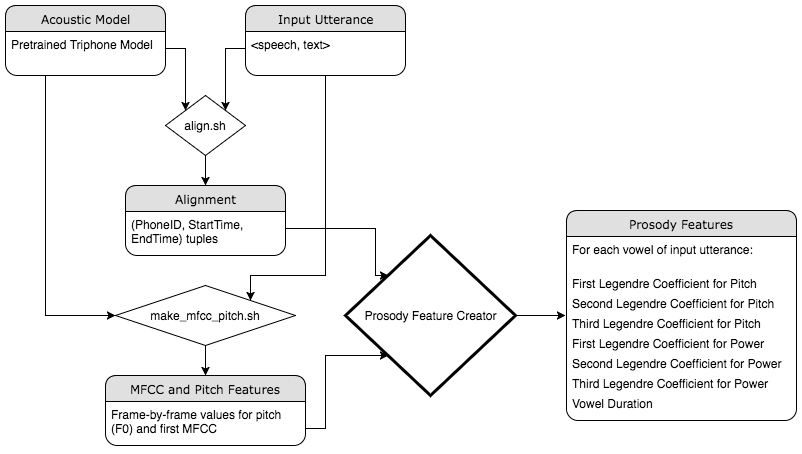
\includegraphics[width=8.5cm]{Prosody_Extraction.png}}
\end{minipage}
\caption{Prosody Feature Extraction}
\label{fig:prosodyextraction}
\end{figure}

First, Kaldi computes a forced alignment of the input audio using a pretrained acoustic triphone model -- in this project, the final triphone model from Kaldi's TEDLIUM recipe -- resulting in a sequence of \textit{(phone\_id, start\_time, end\_time)} tuples.
Next, Kaldi computes the MFCC and pitch features for each frame of the input audio. Finally, the system developed here computes seven real-valued features for each vowel phone in the alignment.

The first three features are the coefficients of the second-degree Legendre series that is the least-squares fit to a series of $(x, y)$ points where the length of the series is the computed number of frames plus 4, the $x$ values are evenly spaced between -1 and 1, and the $y$ values are the frame-by-frame pitch values computed using Kaldi's pitch-extraction algorithm, starting two frames before the beginning of the phone and ending two frames after the end of the phone.
Since Kaldi's algorithm already normalizes the pitch contour over a three-second window, no further normalization is done before computing the Legendre coefficients.

The next three features are the Legendre coefficients for the power (first MFCC component), calculated in the same way as for the pitch features. Since this component is not normalized by Kaldi, my system normalized the coefficient to have mean zero and unit variance over the whole utterance before computing these coefficients.
The seventh feature is simply the duration of the phone.

These seven features were chosen in the hopes of maximizing the useful prosodic information available in a small set of numbers per phoneme.
The two frames (20 ms) before and after the utterance are added to the sequence to improve the conditioning of the least-squares fit matrix; to compensate for potential slight errors in the alignment as computed by Kaldi; and to provide a small degree of context for the vowel in question.
The domain is fixed at [-1, 1] so that the coefficients capture the level, slope and curvature over the length of the phoneme, regardless of the duration.

Most importantly, these features are intended to be useful for identifying which syllables in an utterance are stressed. However, spoken English uses pitch contour to convey more information than simply which syllable is a word is stressed. Pierrehumbert \cite{pierrehumbert1980phonology} identifies 22 different patterns that an English phrase can exhibit, consisting of various combinations of pitch accent, phrase accent, and intonation occurring at the end of a phrase.
These phrases carry semantic content beyond the actual words of the text. For example, different stress patterns can indicate surprise, emphasis, disbelief, or neutrality, among others.

Figure \ref{fig:pitchpow1} displays the pitch and power contours that Kaldi computes for two pronunciations of the two-word phrase ``another orange'' (the phrase is from \cite{pierrehumbert1980phonology}.) In the first audio file, the words are spoken with a tone of disbelief, i.e., ``aNOTHer orange???''. In the second pronunciation, the words are spoken with a neutral tone. The seven computed features for each vowel are displayed in Table \ref{table:pitchpow1}.

\begin{figure}[htb]

\begin{minipage}[b]{.46\linewidth}
  \centering
  \centerline{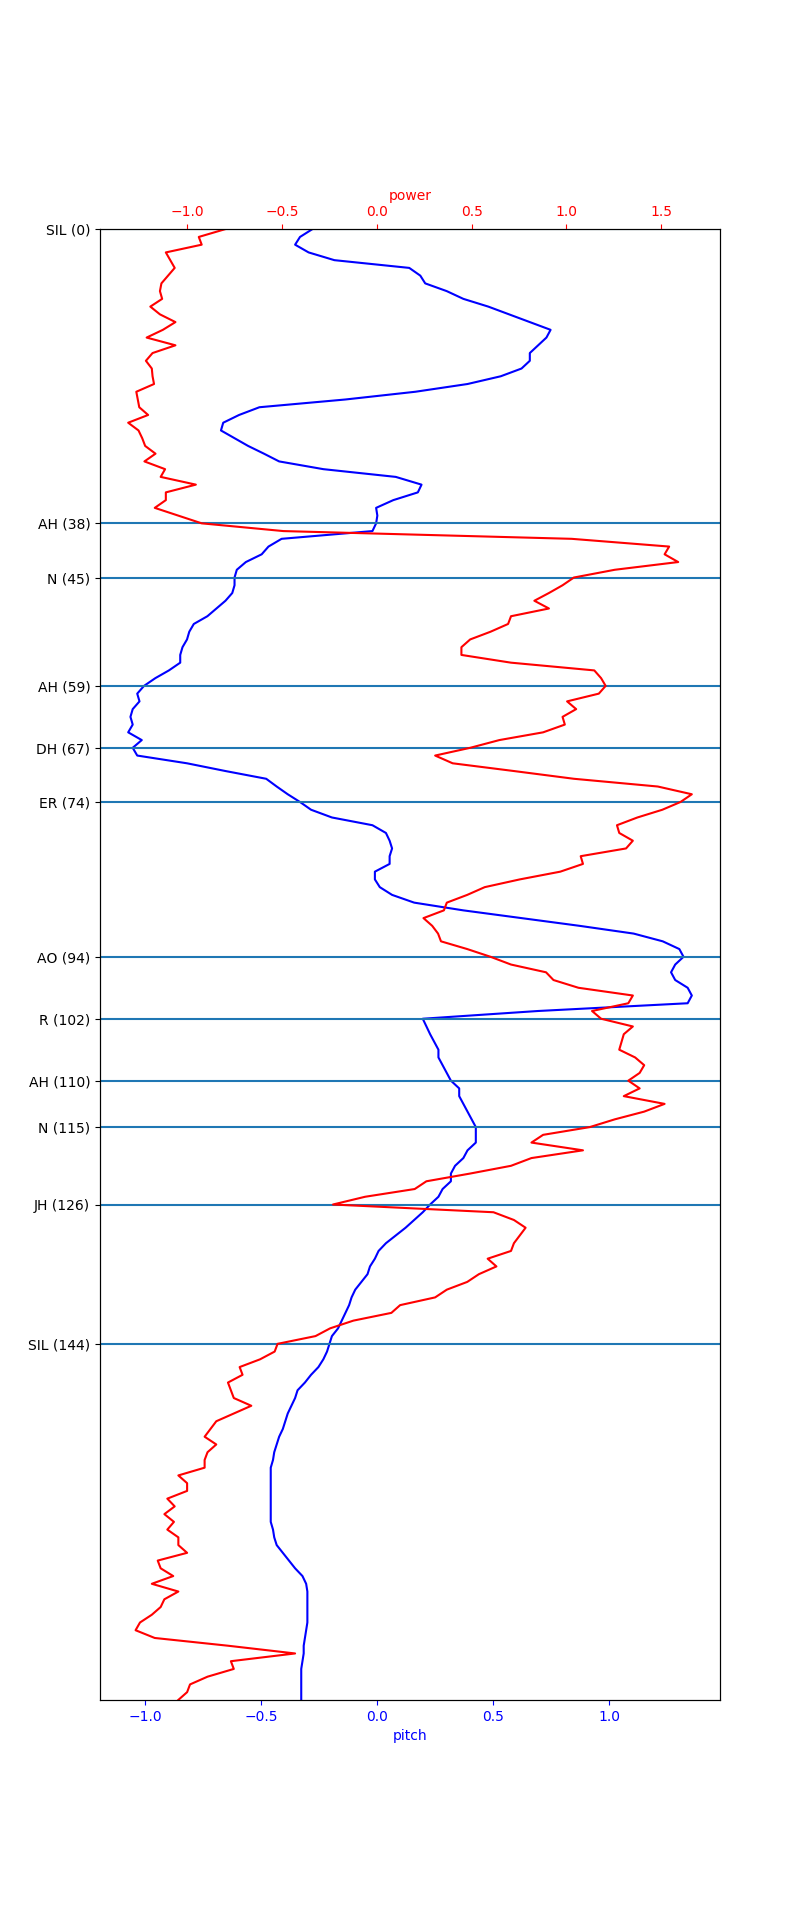
\includegraphics[width=4.0cm]{orange_aNOTHer}}
\end{minipage}
\hfill
\begin{minipage}[b]{0.5\linewidth}
  \centering
  \centerline{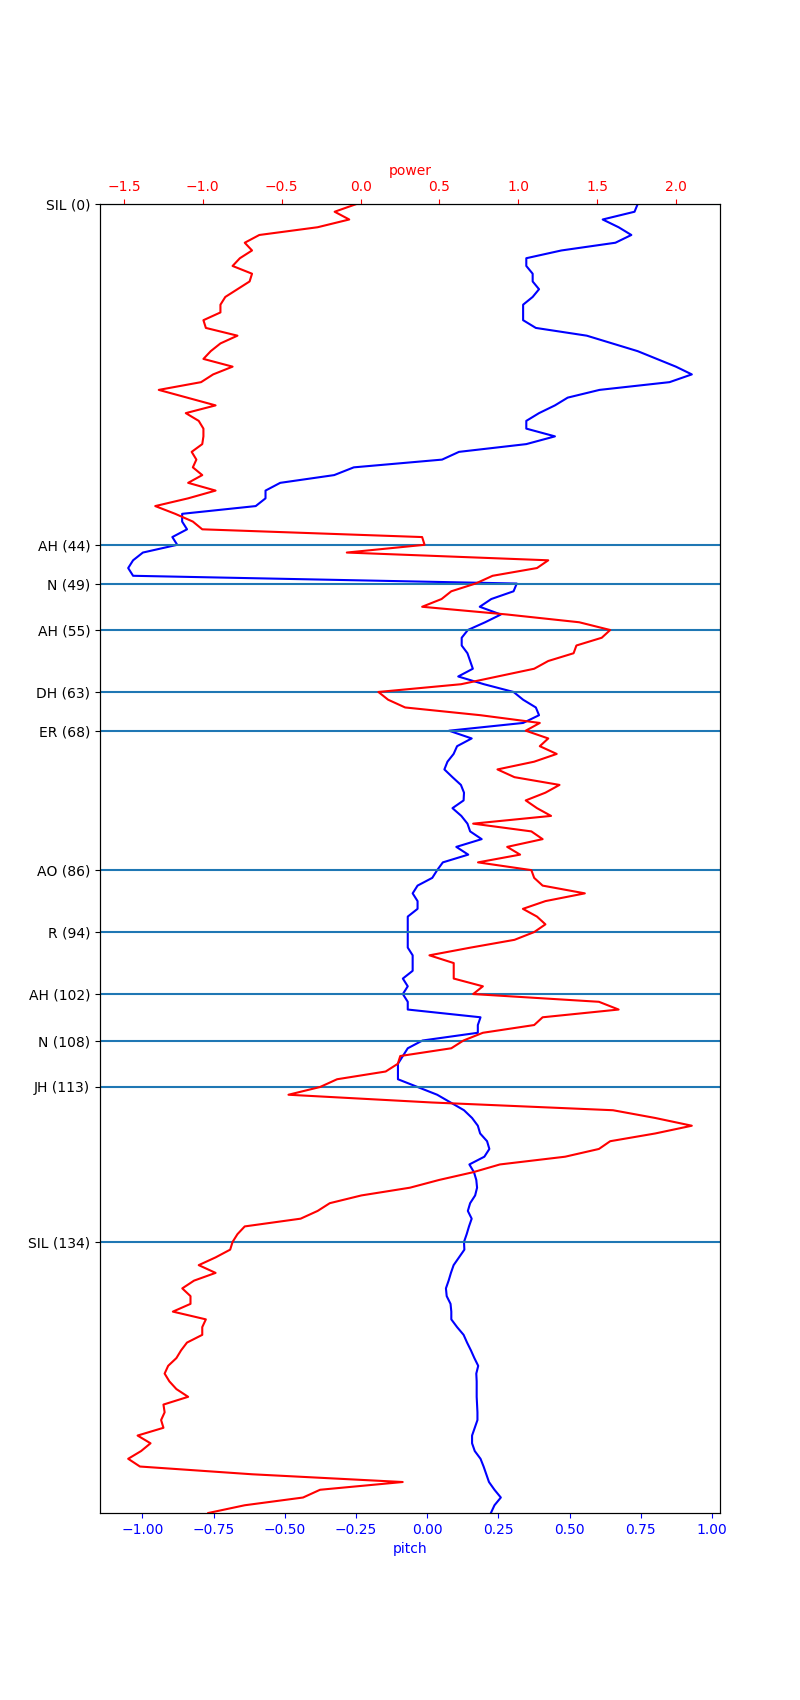
\includegraphics[width=4.5cm]{orange_neutral}}
\end{minipage}
%
\caption{Normalized pitch and power contours. The figure on the left was uttered with a tone of disbelief.}
\label{fig:pitchpow1}
%
\end{figure}

\begin{table}[]
\footnotesize
\centering
\begin{tabular}{|p{1cm}|p{1cm}|p{1cm}|p{1cm}|p{1cm}|p{1cm}|}
\hline
\textbf{}              & \textbf{A(n)}  & \textbf{O(th)} & \textbf{E(r)}  & \textbf{O(r)}  & \textbf{A(nge)} \\ \hline
Pitch 1                & -1.1/-2.4      & -3.2/0.6       & 0.9/0.5        & 3.6/0.0        & 1.2/0.1        \\ \hline
Pitch 2                & -2.0/3.5       & 0.0/0.6        & 5.5/-0.1       & -2.5/-0.2      & 0.8/0.8        \\ \hline
Pitch 3                & 0.8/6.3        & 0.6/1.2        & 3.4/0.5        & -5.0/0.5       & -0.1/-1.1      \\ \hline
Power 1                & 0.1/0.0        & 0.8/1.0        & 0.7/1.0        & 0.8/1.1        & 1.5/0.9        \\ \hline
Power 2                & 2.7/1.5        & -0.1/-0.4      & -0.6/0.5       & 1.3/0.6        & 0.2/0.4        \\ \hline
Power 3                & -1.3/-0.6      & 0.4/-0.3       & 1.4/0.7        & 0.5/0.5        & 0.5/-0.4       \\ \hline
Duration               & -0.2/-0.5      & 0.0/0.0        & 2.0/1.6        & 0.0/0.0        & -0.4/-0.4      \\ \hline
\textbf{Cluster} & \textbf{7 / 6} & \textbf{6 / 4} & \textbf{5 / 4} & \textbf{2 / 4} & \textbf{1 / 1} \\ \hline
\end{tabular}
\caption{Extracted prosody features for two pronunciations. The first number in each cell is for the tone of disbelief. The last row shows the cluster label that the vowel was assigned to.}
\label{table:pitchpow1}
\end{table}

\section{Vowel Clustering}
\label{sec:vowels}

To the extent that the seven extracted prosody features for each vowel do indeed convey useful information, there are numerous ways one could imagine using them to ``clone'' an input utterance.
For example, the output of a speech synthesis system could be distorted in some smooth way in order to try and match the pitch and power contours of the entire input audio.
Alternately, they could be used as the inputs to a supervised classification algorithm that learned to classify each syllable as stressed or unstressed, with the help of a manually-annotated dataset.
The system implemented here uses $k$-means, an unsupervised algorithm, to partition the space of features into 8 categorical cluster labels.

As stated in Sec. \ref{sec:overview}, the input to the vowel-cluster training process consists of an acoustic model and a multi-speaker speech dataset, which for this project was a randomly selected 5\% subsample of the TEDLIUM dataset.
The prosody features for each vowel in the dataset are first computed using the acoustic model as described in Sec. \ref{sec:prosody}.
These features are then normalized over the entire dataset to have zero mean and unit variance on a feature-by-feature basis.
Finally, $k$-means clustering with $k$=8 returns eight vectors in $\mathbf{R}^7$ corresponding to the cluster centroids.
The resulting vowel cluster model therefore consists of the scaling factors that normalize each feature of the input dataset and the eight cluster centroids. This portion of the system was implemented in Python 2 (for compatibility with Kaldi) using \texttt{scikit-learn} \cite{scikit-learn}.

There were number of choices involved in how to perform the clustering, which are discussed further in Sec. \ref{ssec:discussvowels}. The pitch and power contours corresponding to each cluster center are displayed in Figure \ref{fig:clustercenters}.

\begin{figure}[htb]

\begin{minipage}[b]{1.0\linewidth}
  \centering
  \centerline{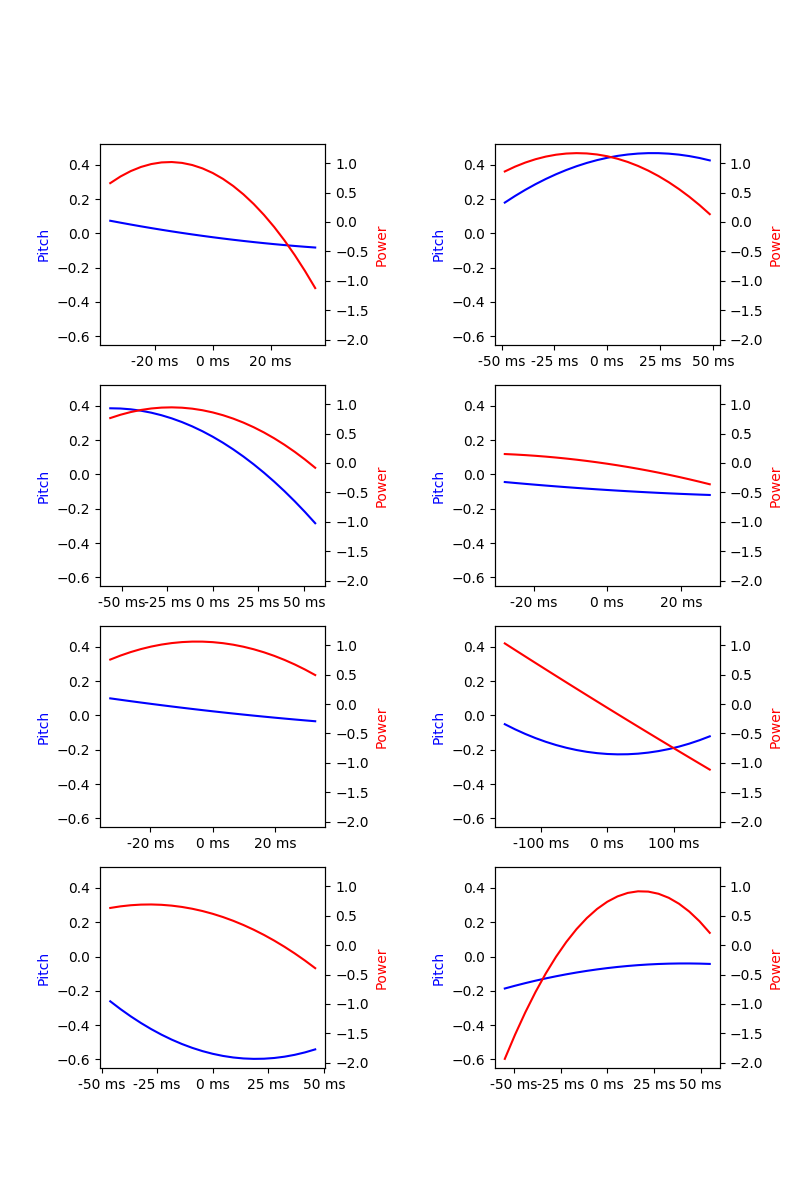
\includegraphics[width=8.5cm]{cluster_centers.png}}
\end{minipage}
\caption{The eight computed cluster centers. Note that while the scale of the y-axis is constant across plots, the contours have different durations.}
\label{fig:clustercenters}
\end{figure}

\section{Speech Synthesis}
\label{sec:tacotron}

The speech-synthesis training portion of the system produces a model that can be used to generate new utterances. The input to this portion of the system is the pretrained acoustic model, the vowel-clustering model resulting from Sec. \ref{sec:vowels}, and a large single-speaker dataset consisting of [text, audio] pairs.
In this phase, the prosody features are first extracted as described in Sec. \ref{sec:prosody}. Next, the vowel-clustering model is used to assign cluster labels to each vowel in the dataset.
The result is a set of [labeled-phone-sequence, audio] pairs; for a single utterance in the dataset, the labeled phone sequence for that utterance is the sequence of phones along with the cluster labels for each vowel. For example, the text for one particularly short utterance in the dataset used here is ``In 1813''.
The corresponding labeled phone sequence is ``IH VOWEL4 N sp SIL EY VOWEL1 T IY VOWEL4 N sp TH ER VOWEL6 T IY VOWEL2 N sp SIL''. The ``sp'' tokens correspond to word boundaries.

The Tacotron \cite{wang2017tacotron} neural network system was trained on the [labeled phone sequence, audio] pairs to produce audio.
Tacotron's internal neural network architecture is far too complex to describe in detail in this paper. As a brief overview, it is based on the Sutskever et al. \cite{sutskever2014sequence} encoder-decoder seq2seq model with Bahdanau \cite{bahdanau2014neural} attention. The input is a sequence of one-hot-encoded characters.
The encoder embeds the characters in a continuous vector space, and passes them through the CBHG module described in the Tacotron paper.
The decoder uses GRUs with attention to produce linear-scale spectrogram as the output sequence. Finally, the Griffin-Lim algorithm produces the actual audio from the spectrogram.

Since Tacotron is agnostic to the character set, the phones and the cluster labels are used here, along with the word-boundary marker, as the character set. Tacotron's neural network architecture makes this possible out-of-the-box; it was specifically designed to accomodate end-to-end training using only audio and the corresponding text as its inputs, in contrast to the relatively complex requirements for most speech synthesis systems.
One specific advantage discussed by the authors is that ``it more easily
allows for rich conditioning on various attributes''. The vowel cluster labels used here are an example of this conditioning.

The ``C'' in CBHG refers to a bank of 1-dimensional convolutional filters; this layer is what allows Tacotron to easily incorporate the vowel markings as if they were simply another character. The convolutional filters include a width of up to 16 characters (in this case, phonemes plus vowel cluster labels), which is more than enough for the model to learn how successive cluster labels are typically associated with the prosody of the training audio.

This project uses Keith Ito's open-source Python 3 / TensorFlow implementation of Tacotron, with only small modifications required to accomodate the modified character set. The model was trained with his LJ Speech Dataset \cite{ljspeech17}, which he describes on his website as follows:
``This is a public domain speech dataset consisting of 13,100 short audio clips of a single speaker reading passages from 7 non-fiction books. A transcription is provided for each clip. Clips vary in length from 1 to 10 seconds and have a total length of approximately 24 hours. The texts were published between 1884 and 1964, and are in the public domain. The audio was recorded in 2016-17 by the LibriVox project and is also in the public domain.''

The result of this portion of the system is a trained model that takes a labeled phone sequence as input and produces audio as output. For this project, the model was trained 200,000 steps, which took approximately five days on a Tesla K80 GPU running on Google Cloud.

\section{New Utterance Generation}
\label{sec:newuttgen}
Once the vowel-cluster and speech synthesis models have been trained, synthesizing new outputs is straightforward.
The only difference at this phase is that Kaldi can optionally be used to generate a transcription before computing the alignments.
Of course, if the input text is provided along with the audio, the alignment will be more accurate.
Once the alignments are computed, the prosody features for the input utterance are extracted as before and the vowel clustering model is then used to assign cluster labels to each vowel.
This sequence of steps results in a labeled phone sequence.
The trained Tacotron model then uses this sequence directly to synthesize a new audio file.

\section{Results and Discussion}
\label{sec:results}

\subsection{Synthesized Audio}
\label{ssec:audio}

Several pairs of input and output audio are included in the repository for this project. For control, audio is also presented which was produced by training a synthesis model on the same phone sequences, but stripped of the vowel cluster numbers and silence tokens.
The results demonstrate, at least to the author's ears, that the extracted features and resulting cluster labels are indeed capturing some semantic meaning in the input that is then reflected in the synthesized audio. In addition, the quality of the audio produced with labels appears to be higher, although this is to be expected.
They also reveal some shortcomings of the approach taken here and possibilities for future improvement.
The synthesized audio all falls within a fairly narrow of output, no matter how dramatically the input differs.
The audio results make it clear that although these cluster labels are a good start, there is room for improvement.
Nevertheless, the audio pairs are distinct enough that a potential controlled experiment is described in Sec. \ref{sec:futurework}. To a certain extent, the narrow output range may reflect the limited emotional range of the speaker in the Tacotron training dataset, who was recorded reading nonfiction books.

\subsection{Vowel Clustering}
\label{ssec:discussvowels}

The number of clusters was chosen somewhat arbitrarily; it was intended to be high enough to distinguish the ways that English speakers pronounce any single vowel in isolation, but low enough that the resulting clusters would generalize well across multiple speakers. Indeed, Pierrehumbert \cite{pierrehumbert1980phonology} distinguishes only between H, L, L+H, and H+L for patterns of the F0 contour.
The use of K-means as opposed to any other unsupervised clustering algorithm was also an arbitrary decision, motivated only by the algorithm's speed and overall good performance on a wide range of clustering tasks.

A second decision was to compute a single set of clusters for all vowels, as opposed to computing clusters for each vowel individually.
Arguments can be made for either choice; to the extent that different vowels have distinct phonetic roles, using a single set of prosody cluster labels for all vowels may inadvertently cause the clusters to distinguish between these vowels instead of between the intended prosodic features. For example, dipthongs may exhibit distinct patterns from monophthongs or the schwa.

\section{Future Work}
\label{sec:futurework}

In addition to exploring alternate clustering algorithms or parameters, one promising approach for future work would be to use a continuous representation of the pitch contour, properly normalized across speakers, as a direct input into the speech synthesis engine.
This might require some modification to the Tacotron architecture, which expects categorical inputs, but the early conversion to embeddings means that continuous inputs could probably be accomodated without too much difficulty.

In addition, the following controlled experiment could be performed with the existing system. First, a set of input audio utterances could be selected for which there is a high degree of listener agreement on either the speaker emotion or on which words were emphasized in the input. Second, two forms of synthesized output could be produced: (a) using the system as described above and (b) trained only on the phone sequences without the SIL or VOWEL tokens.
To the extent that listener agreement on the output audio from (a) matched the original input more than (b), the system could be shown to work or not work accordingly.

\section{Conclusion}
\label{sec:conclusion}
We have described a speech-to-speech pipeline that uses K-means clustering to learn a finite set of suprasegmental features that generalize across multiple speakers. The clusters can be used both to extract a compact representation of prosody from new input utterances and to train a text-to-speech system to incorporate prosody labels into its output. Although the output range is still limited, the resulting audio is distinctly different depending on which clusters are detected in the input.

\section{Acknowledgements}
\label{sec:acknowledgements}
I would like to thank Keith Ito for his outstanding open-source implementation of Tacotron. This project would not have been possible without his work. I would also like to thank Dan Povey, the lead developer of Kaldi, which was also essential to this project. Finally, I would like to thank Professor Beigi for teaching this class. Both the class and this project have been a pleasure!

\bibliographystyle{IEEEbib}
\bibliography{strings,refs}

\end{document}
